\documentclass[dvipdfm,a4paper, 12pt,english]{report}
                                    %romanian
%pentru limba romana
\usepackage{babel}
\usepackage[latin2]{inputenc}
%se pot comenta si elimina (la fel ca si optiunea de mai sus -english) daca textul nu contine diacritice

\usepackage{url}
\usepackage{amssymb}

\usepackage{algorithm}
\usepackage{algorithmicx}
\usepackage{algpseudocode} 
\usepackage{multirow}

\renewcommand{\algorithmiccomment}[1]{\hfill // #1} 

\usepackage{geometry}
\usepackage{graphics}

%\usepackage{color}           %\textcolor{red}{ De completat ... }

%pentru link la citari
\usepackage[dvips]{graphicx,color}
\usepackage[dvipdfm,colorlinks]{hyperref}

\hypersetup{
pdftitle={LucrareLicenta},
pdfauthor={Andreea},
pdfkeywords={pdf, latex, tex, ps2pdf, dvipdfm, pdflatex},
bookmarksnumbered,
pdfstartview={FitH},
urlcolor=blue,
colorlinks=true,
linkcolor=blue,
citecolor=blue,}


\geometry{a4paper,top=2.5cm,left=3cm,right=3cm,bottom=2.5cm}
%controlling the appearance of your headers and footers
\usepackage{fancyhdr}
\pagestyle{fancy}


\lhead{}
\chead{}
\renewcommand{\headrulewidth}{0.2pt}
\renewcommand{\footrulewidth}{0.2pt}



\begin{document}

\begin{titlepage}

	\begin{center}
		\Large{{BABE�-BOLYAI UNIVERISTY CLUJ-NAPOCA}}
		\Large{{FACULTY OF MATHEMATICS AND COMPUTER SCIENCE}}
		
		\vspace{8cm}
		
		\textbf{DIPLOMA THESIS}
		
		\vspace{1cm}
		\Huge\textbf{{DIPLOMA TITLE}}
		\fontsize{12}{14}
		
	\end{center}
	\vspace{6cm}
	
	\hspace*{0.8cm}Supervisor: \hfill  Author: \hspace*{0.8cm} \\    
	\textbf{Prof. Dr. FirstName LastName  \hfill  \textbf{FirstName LastName}}
	
	\vspace{2cm}
	\begin{center}
		\Large{2009}
	\end{center}
\end{titlepage}  
    
    
\newpage
\thispagestyle{empty}
\mbox{}
\newpage
\pagenumbering{roman} 

\renewcommand{\headrulewidth}{0pt}
\renewcommand{\footrulewidth}{0pt}
\cleardoublepage
%\addcontentsline{toc}{Abstract}{\\  Abstract \ . . . . . . . . . . . . . . . . . . . . . . . . . . . . . . . . . . . . . . . . . . . . } 
ABSTRACT
\vspace{0.5cm}	
\hrule
\vspace{0.5cm}	
%\cleardoublepage

Lucr�rile de licen�� vor include un text de o pagin� redactat �n limba englez�, intitulat Abstract, care va con�ine un rezumat pe capitole a lucr�rii de licen�� �i o auto-evaluare a gradului de noutate �i originalitatea lucr�rii, inclusiv cu referire la originalitatea aplica�iei realizate. 

Ultimul paragraf al rezumatului va con�ine urm�torul text: 

This work is the result of my own activity. I have neither given nor received unauthorized assistance on this work. 

Pagina din lucrarea de licen�� care con�ine rezumatul va fi semnat� de student �n original. Studen�ii specializ�rii matematic�-informatic� linia de studiu german� vor redacta acest rezumat �n limba german�. To�i ceilal�i vor redacta rezumatul �n limba englez�. Rezumatele vor fi predate �n format electronic cadrelor didactice �ndrum�toare.


\tableofcontents
           
\newpage
\renewcommand{\headrulewidth}{0.2pt}
\renewcommand{\footrulewidth}{0.2pt}
\pagenumbering{arabic}

\chapter*{Introducere}
\addcontentsline{toc}{chapter}{Introducere} 
 
Absolventul va prezenta rezumativ tema tratat� relativ la enun�ul problemei, obiectivele urm�rite, rolul aplica�iei �i structura lucrarii, precum �i leg�tura dintre capitole.

 
 Lucrarea de fa�� ofer� o vedere de ansamblu a ...
 
Capitolul 2 prezint� ...

�n capitolul 3 sunt definite no�iunile de ...

Capitolul 4 prezint� ...

�n capitolul 5 prezint� ...

Lucrarea se �ncheie cu concluzii �i direc�ii de cercetare.

\chapter{Fundamentarea teoretic�}
\label{CapFT}

Absolventul va prezenta detaliat (pe baza document�rii bibliografice \cite{Crn02}) problematica tratat�:
\begin{itemize}
	\item �ncadrarea temei �ntr-una mai general�;
	\item trecerea �n revist� a abord�rilor existente ale problemei cu marcarea avantajelor �i dezavantajelor;
	\item descompunerea �n subprobleme specifice �i prezentarea modului de rezolvare.
\end{itemize}

	Partea fundament�rii teoretice poate fi consituit� din mai multe capitole, ca de exemplu ``Stadiul actual din domeniu/State of art/Literature Review'' �i ``Modele teoretice �i metode folosite/Research Method'' �i ``Problem Statement''.


\chapter{Dezvoltarea aplicativ�}
\label{CapDA}

Absolventul va prezenta clar partea aplicativ� a lucr�rii �i metodologia de solu�ionare folosind elementele teoretice.

Se va specifica mediul de lucru, a facilit��ilor folosite �n acest mediu, proiectarea aplica�iei, detalii de implementare, exemple de test sau rezultate sub forma unor studii de caz, modul de utilizare a programului 
prin prezentarea documenta�iei de utilizare. Va fi anexat �n lucrare inclusive codul surs�.

Partea dezvolt�rii aplicative poate fi constituit� din mai multe capitole.

Referirea unei figuri \ref{Cap3Figura3-1}.

\begin{figure}[htbp]
	\centering
		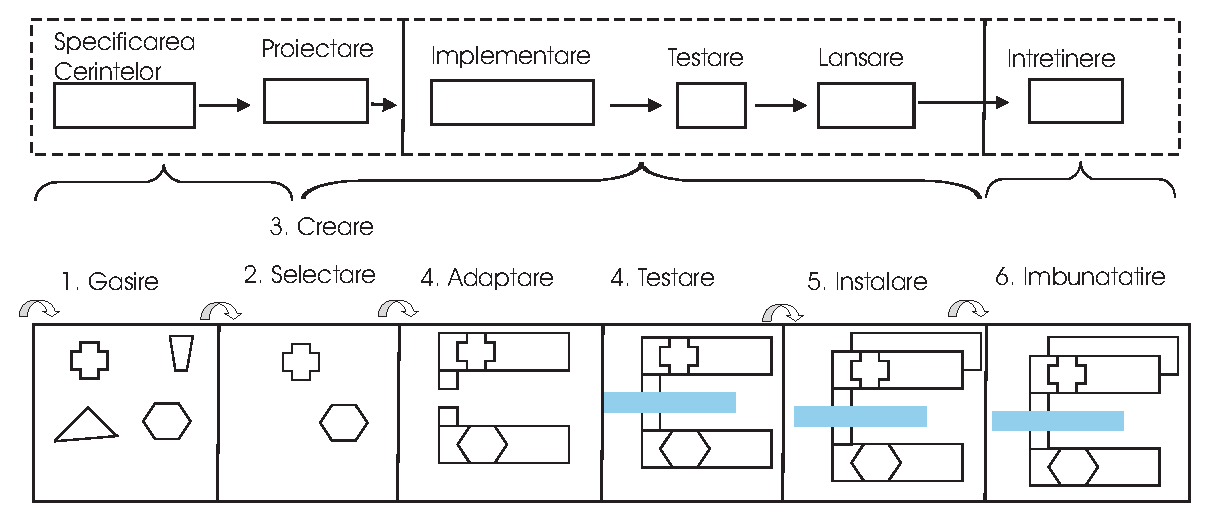
\includegraphics[scale=0.65]{Fig/fig_3_1.eps}
	\caption{Ciclul de dezvoltare al sistemelor bazate pe componente adaptat modelului cascad�}
	\label{Cap3Figura3-1}
\end{figure}


Referirea la Tabelul \ref{Cap3Tabel01}. 

\begin{table}[htbp]
\begin{center}
\begin{tabular}
{||p{100pt}||p{60pt}|p{60pt}||}
\hline
 Nume algoritm& 
 Toate solu�iile &
 Solu�ia optim�\\
\hline 
\hline Nume 1 & $20$ & $5$  \\
\hline Nume 2 & $20$ & $2$  \\
\hline
\end{tabular}
\end{center}
\caption{Solu�ii ob�inute }
\label{Cap3Tabel01}
\end{table}



\section{Prima sec�iune}

\subsection{Subsec�iunea unu}


Exemplu de prezentare algoritm.

\begin{algorithm}[htbp]
\begin{small}
\begin{algorithmic}  
\State \textbf{Input:}
\State {\ $\bullet$ the number $n$ ;}
\State {\ $\bullet$ the list $paramList$ of additional parameters that will be described in the proposed approaches.}
\State \textbf{Output:}
\State {\ $\bullet$ the solution.}
\State{}
\State {\textbf{Subalgorithm} \emph{IterativeBacktracking(n,[$paramListBack$])} is:}
\State \textbf{Begin}   
    \State {Let k := 1; possible[1] := \textit{init(1)};}   \Comment{initialise the search for the index k (=1)}
    \While {($k > 0$)}
    	\State {Let found := \textit{false}; v := possible[k];}
    	\While {( \textit{next(k,v,new)} \textbf{and} (not found))}
    			\State {Let v := new;}
    			\If {(\textit{conditionToContinue(k, possible,v,[$paramListCtC$])})}
    					\State { found := \textit{true};}
    			\EndIf    	
    	\EndWhile    
    	\If {(found)}
    			\State {Let possible[k] := v;}        \Comment{possible[1..k] is a solution candidate}
    			\If {(\textit{solution(n,k,possible,[$paramListSol$])})}          \Comment{found a solution}
    					\State {Print possible[1..k];}
    			\Else
    					\State { Let k := k+1;}     \Comment{step forward on level k+1}
    					\State {possible[k] := init(k);}
    			\EndIf    	
    	\Else
    			\State {k := k-1;}                 \Comment{step backward (backtrack to level k-1)}
    	\EndIf
    \EndWhile   
\State \textbf{End.}
\end{algorithmic}
\end{small}
\caption{The \textit{IterativeBacktracking} subalgorithm }
\label{AlgBackGeneral}
\end{algorithm}

\subsection{Subsec�iunea a doua}

\section{A doua sec�iune}





\chapter{Concluzii finale}
\label{CapCF}

Absolventul va realiza o autoevaluare a rezultatelor prezentate (punctarea aspectelor originale, a avantajelor �i limitelor solutiilor oferite) �i a eventualelor aspecte r�mase nerezolvate,

�n general se prezint� �n urm�toarele subsec�iuni: Concluzii, Sumarul contribu�iilor, Direc�ii viitoare de cercetare.

\section{Concluzii}

\section{Contribu�ii}

\section{Direc�ii viitoare de cercetare}



%ca sa apara bibliografia in contents
\clearpage
\addcontentsline{toc}{chapter}{Bibliografy}



\appendix

\chapter{Documente de analiz� �i proiectare}

\section{Documente de analiz�}

\section{Documente de proiectare}


\chapter{Cod surs�}

%\section{Anumite p�r�i de cod surs�}

%\chapter{Manualul de utilizare}

%\section{Func�ionalit��i principale }

%\section{Alte func�ionalit��i }



\bibliographystyle{alpha}
\bibliography{BiblioLicenta}

\end{document}